\section{Introduction}

very briefly summarize main behavioral findings, cite behavioral summary in sc paper, then go on to cite preprint stating that it contains a shorter summary of the longer results in SC paper and may interest the reader.

summarize Mean Ratings, Duration, Touches and Distance-covered between touches map as behavioral results. Refer to statistical results given in preprint?

Then present EEG findings of the one main cluster of interest, power spectrum ANOVA and regression as well as ERSP ANOVA and regression

Argumentation:
Show that ITI (Inter touch Interval) correlates:
with the location in the maze (low ITI in corners / high ITI along straight segments)
if TRUE: make heatmap with CDATA of ITI (cold color = high ITI, warm color = low ITI)
with the amount of heading change (heading changes vs. maintaining heading)
Single-trial regression of ITI in ERSP controlling for touch duration and run (ignore study design) since run causes a decrease in ITI.
Summarize group-level average (can simply average across betas since ITI is zscored) across subjects and check if TFCE statistic is significant
Do that for different clusters (test if response between clusters differ?), RSC - parietal - occipital


\begin{comment}
Below is the list of the general idea for the data analysis:
\begin{itemize}
    \item ACC related trials mit bewegungsparameter, error detection klar: ACC ist region of interest, error detection vs. bewegungsparameter
    \item Avinash hatte daran gearbeitet: Velocity Parameter in Sydney Datensatz bewerten, noch nicht fertig, frage nach. velocity, beschleunigung, reaktionszeit
    \item höhere varianz mit höhere geschwindigkeit mehr slag im system -> erp effect velocity, beschleunigung, reaktionszeit
    \item vergleich efferent copy und motor feedback => wie lang dieser vergleich zeit in anspruch nimmt, wird prädizieren, ob erp amplitude davon beeinflusst wird.
    \item 3 positionen von cube -> nicht genug trials um das als faktor zu untersuchen
    \item nachträglich wäre erst interessant was nach Error detection passiert, vermutlich wird das parietal passieren. gibt es Potenzial andere areale, die damit zusammenhängen? interaktionsanalyse: höhere precision auch bei höheren geschwindigkeit durch additional sensorischen feedback / bei erhöhter immersion abhängiger maß: velocity auf erp mean von beta-erp für visual und visual vibro
    \item follow-up analysis: einfluss auf latenz: nicht klar zu definieren., reaktionszeit -> nachgeordnete Fragestellung
\end{itemize}

Below is the raw list of data processing:
\begin{itemize}
    \item ICA and preprocessing according to bemobil pipeline
    \item study level clustering based on ROI located at ACC (holroyd \& thorsten's Paper : region of interest for ACC)
    \item clean mismatch epochs with eeglabs autorej function (8 Durchgänge, 10\% der Trials sind dann gereinigt)
    \item baseline of mismatch ERP: select 300 ms time window after trial is started and participant wait at least 1s for box to appear (includes motor readiness potential von resting zu starting point, starting point ist näher am signal und hat relevanterer Aktivität; den starting point als 0 und dann subtraktive single trial baseline berechnung anstelle average baseline, was dann als signal sauberer waere)
    \item single trial velocity parameters von Einzel-ERPs
\end{itemize}
\end{comment}



  \begin{minipage}[]{\textwidth}
    \begin{flushleft}\textbf{B}\end{flushleft}
    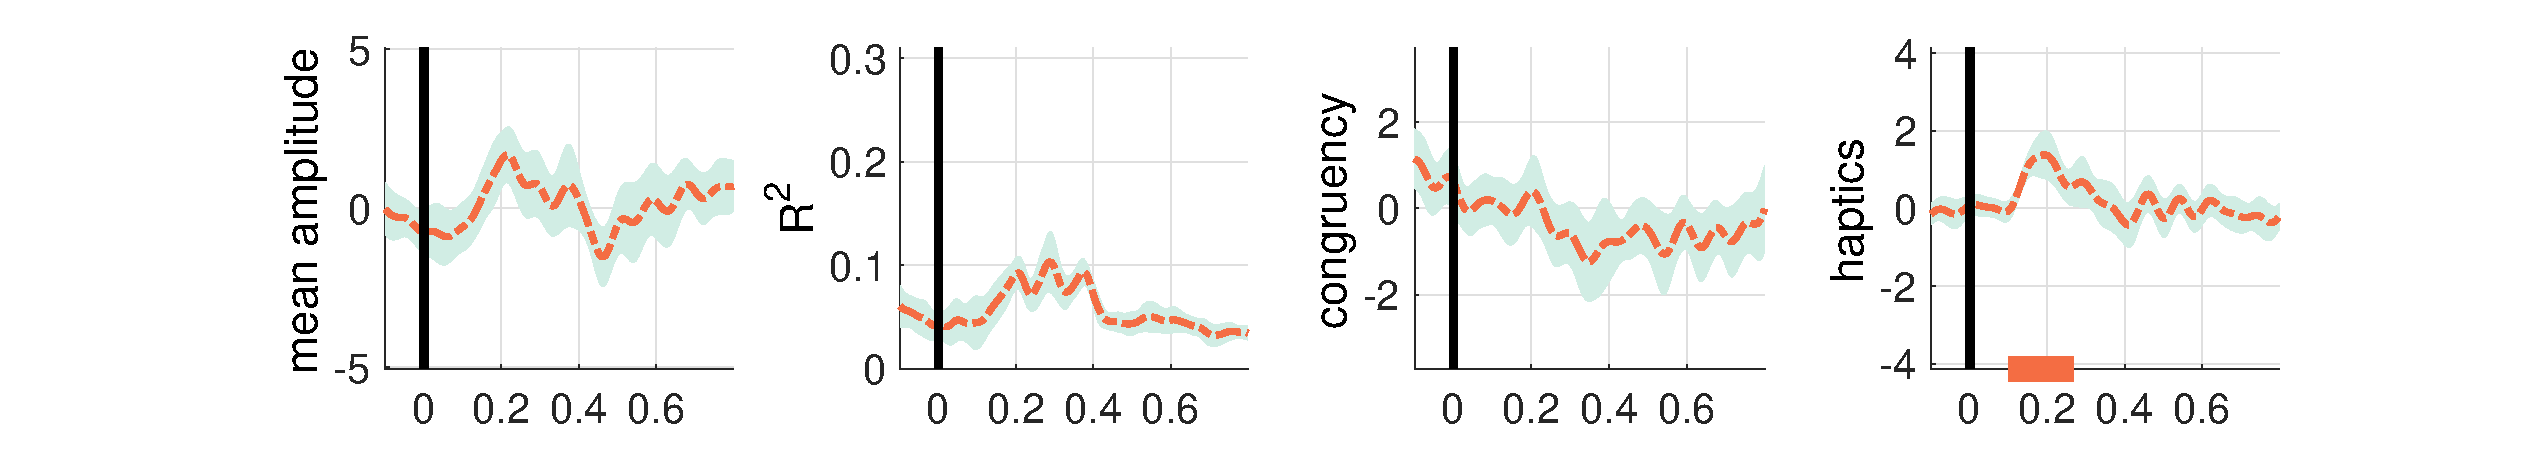
\includegraphics[width=\textwidth]{figures/erp_congruency_Pz.eps}
    \label{erp_Pz}
  \end{minipage}
  \label{erps}